%%%%%%%%%%%%%%%%%%%%%%%%%%%%%%%%%%%%%%%%%%%%%%%%%%
%	JASA LaTeX Template File
%  For use in making articles using JASAnew.cls
% July 26, 2017
%%%%%%%%%%%%%%%%%%%%%%%%%%%%%%%%%%%%%%%%%%%%%%%%%%

%% Step 1:
%% Uncomment the style that you want to use:

%%%%%%% For Preprint
%% For manuscript, 12pt, one column style

%% Comment this out if you'd rather use another style:
\documentclass[preprint]{JASAnew}

%%%%% Preprint Options %%%%%
%% The track changes option allows you to mark changes
%% and will produce a list of changes, their line number
%% and page number at the end of the article.
%\documentclass[preprint,trackchanges]{JASAnew}

%% authaffil option will make affil immediately
% follow author, otherwise authors are grouped, and affiliations
% are stacked underneath all the authors.
%\documentclass[preprint,authaffil]{JASAnew}

%% NumberedRefs is used for numbered bibliography and citations.
%% Default is Author-Year style.
%% \documentclass[preprint,NumberedRefs]{JASAnew}

%%%%%%% For Reprint
%% For appearance of finished article; 2 columns, 10 pt fonts

% \documentclass[reprint]{JASAnew}

%%%%% Reprint Options %%%%%

%% For testing to see if author has exceeded page length request, use 12pt option
%\documentclass[reprint,12pt]{JASAnew}

% authaffil option will make affil immediately
% follow author, otherwise authors are grouped, and affiliations
% are stacked underneath all the authors.
%\documentclass[reprint,authaffil]{JASAnew}

%% NumberedRefs is used for numbered bibliography and citations.
%% Default is Author-Year style.
% \documentclass[reprint,NumberedRefs]{JASAnew}

%% TurnOnLineNumbers
%% Make lines be numbered in reprint style:
% \documentclass[reprint,TurnOnLineNumbers]{JASAnew}

\usepackage{fontspec}

    \setmainfont[]{Times New Roman}

\usepackage{natbib}


\usepackage{cleveref}
\usepackage{ctable}
\usepackage[caption=false]{subfig}
\usepackage{enumerate}

\begin{document}
%% the square bracket argument will send term to running head in
%% preprint, or running foot in reprint style.

\title[Voicing-related differences in vowel duration as compensatory temporal
adjustment]{Voicing-related differences in vowel duration as compensatory temporal
adjustment: An exploratory study of the voicing effect in Italian and
Polish}

% ie
%\title[JASA/Sample JASA Article]{Sample JASA Article}

%% repeat as needed

\author{Stefano Coretta}
% ie
%\affiliation{Department1,  University1, City, State ZipCode, Country}
\affiliation{Linguistics and English Language, University of Manchester, Oxford Road,
Manchester, M13 9PL, United Kingdom}
%% for corresponding author
\email{stefano.coretta@manchester.ac.uk}
%% for additional information


% ie
% \author{Author Four}
% \email{author.four@university.edu}
% \thanks{Also at Another University, City, State ZipCode, Country.}

%% For preprint only,
%  optional, if you want want this message to appear in upper left corner of title page
% \preprint{}

%ie
%\preprint{Author, JASA}

% optional, if desired:
%\date{\today}

\begin{abstract}
% Put your abstract here. Abstracts are limited to 200 words for
% regular articles and 100 words for Letters to the Editor. Please no
% personal pronouns, also please do not use the words ``new'' and/or
% ``novel'' in the abstract. An article usually includes an abstract, a
% concise summary of the work covered at length in the main body of the
% article.
Over a century of phonetic research have established the
cross-linguistic existence of the so called `voicing effect', by which
vowels tend to be shorter when followed by voiceless stops and longer
when the following stop is voiced. However, no agreement is found among
scholars regarding the source of this effect, and several causal
accounts have been advanced. A notable one is the compensatory temporal
adjustment account, according to which the duration of the vowel is
inversely correlated with the stop closure duration (voiceless stops
having longer closure durations than voiced stops). The compensatory
account has been criticised due to lack of empirical support and its
vagueness regarding the temporal interval within which compensation is
implemented. The results from this exploratory study of Italian and
Polish suggest that the duration of the interval between two consecutive
stop releases in CVCV words in these languages is not affected by the
voicing of the second stop. The durational difference of the first vowel
then follows from differences in closure durations of the following
stop. It is proposed that these findings agree with a gestural
organisation in which the right edge of the consonant is in a constant
relationship with the preceding vowel.
\end{abstract}

%% pacs numbers not used

\maketitle

%  End of title page for Preprint option --------------------------------- %

%% See preprint.tex/.pdf or reprint.tex/.pdf for many examples


%  Body of the article
\section{Introduction}\label{introduction}

\label{s:intro}

Almost a hundred years of research have consistently shown that
consonantal voicing has an effect on preceding vowel duration: vowels
followed by voiced obstruents are longer than when followed by voiceless
ones
\citep{meyer1904, heffner1937, house1953, belasco1953, peterson1960, halle1967, chen1970, klatt1973, lisker1974, raphael1975, javkin1976, maddieson1976, farnetani1986, kluender1988, laeufer1992, fowler1992, hussein1994, esposito2002, lampp2004, warren2005, durvasula2012}.
This so called `voicing effect' has been found in a considerable variety
of languages, including (but not limited to) English, German, Hindi,
Russian, Italian, Arabic, and Korean (see \citealt{maddieson1976} for a
more comprehensive, but still not exhaustive list). Despite of the
plethora of evidence in support of the \emph{existence} of the voicing
effect, agreement hasn't been reached regarding its \emph{source}.

Several proposals have been put forward in relation to the possible
source of the voicing effect (see \citealt{soskuthy2013} and
\citealt{begus2017} for an overview). The majority of the proposed
accounts place the source of the voicing effect in properties of speech
production.\footnote{Two accounts that posit a perceptual cause are \citet{javkin1976} and \citet{kluender1988}. To the best of my knowledge, Javkin's (1976) proposal remains to be empirically tested, while see \citet{fowler1992} for arguments against \citet{kluender1988}.}
A notable production account, which will be the focus of this study, is
the compensatory temporal adjustment account
\citep{lindblom1967, slis1969a, slis1969, lehiste1970, lehiste1970a}.
According to this account, the voicing effect follows from the
reorganisation of gestures within a unit of speech that is not affected
by stop voicing. The duration of such unit is held constant across
voicing contexts, while the duration of voiceless and voiced obstruents
differs. It is well known that the closure of voiceless stops is longer
than that of voiced stops
\citep{lisker1957, van-summers1987, davis1989, de-jong1991}. As a
consequence, vowels followed by voiceless stops (which have a long
closure) are shorter than vowels followed by voiced stops (which have a
short closure). Advocates of the compensatory account propose two
prosodic units as the scope of the temporal adjustment: the syllable
(or, more neutrally, the VC sequence, \citealt{lindblom1967}), and the
word \citep{slis1969a, slis1969, lehiste1970, lehiste1970a}. However,
the compensatory temporal adjustment account has been criticised in
subsequent work.

Empirical evidence and logic challenge the proposal that the syllable or
the word have a constant duration and hence drive compensation. First,
Lindblom's \citet{lindblom1967} argument that the duration of the
syllable is constant is not supported by findings in \citet{chen1970}
and \citet{jacewicz2009}. \citet{chen1970} rejects a syllable-based
compensatory account on the light of the fact that the duration of the
syllable is affected by consonant voicing. \citet{jacewicz2009} further
show that the duration of monosyllabic words in American English changes
depending on the voicing of the coda consonant. Second, although the
results in \citet{slis1969} suggest that the duration of disyllabic
words in Dutch is constant whether the second stop is voiceless or
voiced, it does not follow from this fact that compensation should
necessarily target the vowel preceding the stop. Indeed, it is logically
possible that the following unstressed vowel could be the target of the
compensation, therefore differences in preceding vowel duration still
call for an explanation.

The compensatory temporal adjustment account has been further challenged
on the basis of the so called `aspiration effect' \citep{maddieson1976},
by which vowels are longer when followed by aspirated stops than when
followed by non-aspirated stops. In Hindi, vowels before voiceless
unaspirated stops are the shortest, followed by vowels before voiced
unaspirated and voiceless aspirated stops, which have similar duration,
followed by vowels before voiced aspirated stops, which are the longest.
\citet{maddieson1976} find no compensatory pattern between vowel and
consonant duration: the consonant /t/, which has the shortest duration,
is preceded by the shortest vowel, and vowels before /d/ and /tʰ/ have
the same duration although the durations of the two consonant are
different. \citet{maddieson1976} argue that a compensatory explanation
for differences in vowel duration cannot be maintained.

However, a re-evaluation of the way consonant duration is measured in
\citet{maddieson1976} might actually turn their findings in favour of a
compensatory account. Due to difficulties in detecting the release of
the consonant of interest, consonant duration in \citet{maddieson1976}
is measured from the closure of the relevant consonant to the release of
the following, (e.g., in \emph{ab sāth kaho}, the duration of /tʰ/ in
\emph{sāth} was calculated as the interval between the closure of /tʰ/
and the release of /k/). This measure includes the burst and aspiration
(if present) of the consonant following the target vowel.
\citet{slis1969a}, however, state that the inverse correlation between
vowel duration and the following consonant applies to \emph{closure}
duration, and not to the entire \emph{consonant} duration. If a
correlation exists between vowel and closure duration, the inclusion of
burst and/or aspiration clearly alters this relationship.

Indeed, the study on Hindi voicing and aspiration effects conducted by
\citet{durvasula2012} indicates that closure duration, measured from
closure onset to closure offset, decreases according to the hierarchy
voiceless unaspirated \textgreater{} voiced unaspirated \textgreater{}
voiceless aspirated \textgreater{} voiced aspirated, which closely
resembles the order of increasing vowel duration in
\citet{maddieson1976}. Nonetheless, \citet{durvasula2012} do not find a
negative correlation between vowel duration and consonant closure
duration, but rather a (small) \emph{positive effect}. Vowel duration
increases with closure duration when voicing and aspiration are taken
into account. However, as noted in \citet{begus2017}, it is likely that
this result is a consequence of not controlling for speech rate. A small
negative effect of closure duration can turn positive if the effect of
speech rate (which is positive) is greater, given the cumulative nature
of these effects \citep[p. 2177]{begus2017}.

Further evidence for a compensatory account comes from the effect of a
third type of consonants, namely ejectives. \citet{begus2017} finds that
in Georgian (which contrasts aspirated, voiced, and ejective consonants)
vowels are short when followed by voiceless aspirated stops, longer
before ejective stops, and longest when followed by voiced stops.
Crucially, stop closure duration follows the reversed pattern: closure
duration is short in voiced stops, longer in ejectives, and longest in
voiceless aspirated stops. Moreover, vowel duration is inversely
correlated with closure duration across the three phonation types.
\citet{begus2017} argues that these findings support a temporal
compensation account (although not univocally, see
\citealt[Section V]{begus2017}).

To summarise, a compensatory temporal adjustment account has been
proposed to explain the voicing effect. According to such account, the
difference in vowel duration before consonants varying in voicing (and
possibly other phonation types) is the outcome of a compensation between
vowel and closure duration. After a careful review of the critiques
advanced by \citet{chen1970} and \citet{maddieson1976}, and in face of
the results in \citet{slis1969} and \citet{begus2017}, a compensatory
account gains credibility. However, issues about the actual
implementation of the compensation mechanism still remain. In
conclusion, while the compensatory temporal adjustment account is
plausible on the light of the reviewed literature, we are left with the
necessity of finding a constant speech interval within which
compensation is logically implemented.

\subsection{The present study}\label{the-present-study}

This paper reports on selected results from a broader exploratory study
that investigates the relationship between vowel duration and consonant
voicing from both an acoustic and articulatory perspective. Synchronised
recordings of audio, ultrasound tongue imaging, and electroglottography
were carried out to enable a data-driven approach to the analysis of
features related to the voicing effect in the context of disyllabic
(CV́CV) words in Italian and
Polish.\footnote{As per \citet{cysouw2013}, the glossonyms \textit{Italian} and \textit{Polish} as used here refer, respectively, to the languoids Italian [\textsc{Glottocode}: \texttt{ital1282}] and Polish [\textsc{Glottocode}: \texttt{poli1260}].}
Given its exploratory nature, this study was not devised to test the
compensatory account, but rather to collect articulatory and acoustic
data on the voicing
effect.\footnote{To the best of my knowledge, this is the first attempt to gather synchronised acoustic, tongue imaging and electroglottographic data in relation to the voicing effect.}
Moreover, the design of the study has been constrained by the use of
such articulatory techniques (see \Cref{s:method}). Since the tongue
imaging and electroglottographic data don't bear on the main argument
put forward here, only the results from acoustics will be discussed.

Italian and Polish reportedly differ in the magnitude of the effect of
stop voicing on vowel duration. Italian has been unanimously reported as
a voicing-effect language
\citep{caldognetto1979, farnetani1986, esposito2002}. The mean
difference in vowel duration when followed by voiceless vs.~voiced
consonants ranges between 22 and 24 ms, with longer vowels followed by
voiced
consonants.\footnote{The mean differences are based on 3 speakers in \citealt{farnetani1986} and 7 speakers in \citealt{esposito2002}. \citealt{caldognetto1979} does not report estimates of vowel duration, but the study is based on 10 speakers.}
On the other hand, the results regarding the presence and magnitude of
the effect in Polish are mixed. While \citet{keating1984} reports no
effect of voicing on vowel duration in data from 24 speakers,
\citet{nowak2006} finds that vowels followed by voiced stops are 4.5 ms
longer in the 4 speakers recorded. Moreover, \citet{malisz2008} argue
based on data from 40 speakers that the magnitude of the voicing effect
in Polish is highly idiosyncratic, and claim their results are
inconclusive on this matter.

The acoustic data from the exploratory study discussed here confirms the
existence of a voicing effect in Italian and Polish, and suggests that
the duration of the interval between two consecutive stop releases (the
Release to Release interval) is not affected by the voicing of the
second consonant in both languages. This finding is compatible with a
compensatory temporal adjustment account by which the timing of the stop
closure onset within said interval determines the respective durations
of vowel and closure. I further propose that the constant duration of
the Release to Release interval is congruent with current views on
gestural timing \citep{goldstein2014} and I discuss the insights such an
account provides in relation to our understanding of the gestural
organisation of speech.

\section{Method}\label{method}

\label{s:method}

\subsection{Participants}\label{participants}

Seventeen subjects in total participated in this exploratory study.
Eleven subjects are native speakers of Italian (5 female, 6 male), while
six are native speakers of Polish (3 female, 3 male). The Italian
speakers are from the North and Centre of Italy (8 speakers from
Northern Italy, 3 from Central Italy). The Polish group has 2 speakers
from Western Poland, 3 speakers from Central Poland, and 1 speaker from
Eastern Poland. For more information on the sociolinguistic details of
the speakers, see \Cref{a:socioling}. Ethical clearance for this study
was obtained from the University of Manchester (REF 2016-0099-76). The
participants signed a written consent and received a monetary
compensation of £10.

\subsection{Equipment}\label{equipment}

The acquisition of the audio signal was achieved with the software
Articulate Assistant Advanced™ (AAA, v2.17.2, \citealt{articulate2011})
running on a Hawlett-Packard ProBook 6750b laptop with Microsoft Windows
7. Audio recordings were sampled at 22050 MHz (16-bit), in a proprietary
format (\texttt{.aa0}). A FocusRight Scarlett Solo pre-amplifier and a
Movo LV4-O2 Lavalier microphone were used for audio recording. The
microphone was placed at the level of the participant's mouth on one
side, at a distance of about 10
cm.\footnote{The microphone was clipped onto a metal headset wore by the participant, which is part of the ultrasound equipment.}

\subsection{Materials}\label{materials}

\label{s:materials}

The target stimuli were disyllabic words with
C\textsubscript{1}V\textsubscript{1}C\textsubscript{2}V\textsubscript{2}
structure, where C\textsubscript{1} = /p/, V\textsubscript{1} = /a, o,
u/, C\textsubscript{2} = /t, d, k, g/, and V\textsubscript{2} =
V\textsubscript{1} (e.g. /pata/, /pada/, /poto/,
etc.).\footnote{Italian has both a mid-low [ɔ] and a mid-high [o] back vowel in its vowel inventory. These vowels are traditionally described as two distinct phonemes \citep{kramer2009}, although both their phonemic status and their phonetic substance are subject to a high degree of geographical and idiosyncratic variability \citep{renwick2016}. As a rule of thumb, stressed open syllables in Italian (like the ones used in this study) have [ɔː] (vowels in penultimate stressed open syllables are long) rather than [oː] \citep{renwick2016}. On the other hand, Polish has only a mid-low back vowel phoneme /ɔ/ \citep{gussmann2007}. For sake of typographical simplicity, the symbol /o/ will be used here for both languages.}
Most are nonce words, although inevitably some combinations produce real
words both in Italian (4 words) and Polish (2 words, see
\Cref{a:targets}). The lexical stress of the target words was placed by
speakers of both Italian and Polish on V\textsubscript{1}, as intended.

The make-up of the target words was constrained by the design of the
experiment, which included ultrasound tongue imaging (UTI). Front vowels
are difficult to image with UTI, since their articulation involves
tongue positions which are particularly far from the ultrasonic probe,
hence reducing the visibility of the tongue contour. For this reason,
only central and back vowels were included. Since one of the variables
of interest in the exploratory study was the closing gesture of
C\textsubscript{2}, only lingual consonants were used. A labial stop was
chosen as the first consonant to reduce possible coarticulation with the
following vowel (although see \citealt{vazquez-alvarez2007}).

The target words were embedded in a frame sentence, \emph{Dico X
lentamente} `I say X slowly' in Italian \citep[following][]{hajek2008},
and \emph{Mówię X teraz} `I say X now' in Polish, and presented
according to the respective writing conventions. These sentences were
chosen in order to keep the placement of stress and emphasis similar
across languages.

\subsection{Procedure}\label{procedure}

The participant was asked to read the sentences with the target words
which were sequentially presented on the computer screen. The order of
the sentences was randomised for each participant. Participants read the
list of randomised sentence stimuli 6 times. Due to software
constraints, the order of the list was kept the same across the six
repetitions within each participant. The reading task lasted between 15
and 20 minutes, with optional short breaks between one repetition and
the other. The total experiment time lasted around 45 minutes. Each
speaker read a total of 12 sentences for 6 times (with the exceptions of
IT02, who repeated the 12 sentences 5 times, and IT07, with whom words
containing /u/ were not recorded due to technical difficulties relating
to ultrasound data collection), which yields to a grand total of 1224
tokens (792 from Italian, 432 from
Polish).\footnote{IT01 and IT02 (the first two participants of this study) also read sentences with words starting with /b/, which were later excluded from the experimental design. The data from /b/-initial words are not included in the analysis reported in this paper.}

The experiment was carried out in two locations: in the sound attenuated
booth of the Phonetics Laboratory at the University of Manchester, and
in a quiet room in a field location in Italy (Verbania, Northern Italy).
In both locations the equipment and procedures were the same. Data
collection started in December 2016 and ended in March 2018.

\subsection{Data processing and
measurements}\label{data-processing-and-measurements}

\ctable[caption = List of measurements as extracted from acoustics.,
label = t:dur-measures,
width=\textwidth,
star
]{ll>{\raggedright}p{9cm}}{}{
\FL
\textbf{landmark}               &                  & \textbf{criteria}                                                                                    \ML
vowel onset           & (V1 onset)         & appearance of higher formants in the spectrogram following the release of /p/ (C1)            \NN
vowel offset          & (V1 offset)        & disappearance of the higher formants in the spectrogram preceding the target consonant (C2) \NN
consonant onset       & (C2 onset)         & corresponds to V1 offset                                                                    \NN
closure onset         & (C2 closure onset) & corresponds to V1 offset                                                                    \NN
consonant offset      & (C2 offset)        & appearance of higher formants of the vowel following C2 (V2); corresponds to V2 onset                                \NN
consonant release & (C1/C2 release)         & automatic detection + manual correction \citep{ananthapadmanabha2014}                                           \LL
}

The audio recordings were exported from AAA in \texttt{.wav} format at
the same sample and bit rate for further processing. A forced aligned
transcription was accomplished through the SPeech Phonetisation
Alignment and Syllabification software (SPPAS) \citep{bigi2015}. The
outcome of the automatic annotation was manually corrected, according to
the criteria in \Cref{t:dur-measures}. The releases of C1 and C2 were
detected automatically by means of a Praat scripting implementation of
the algorithm described in \citet{ananthapadmanabha2014}. The durations
in milliseconds of the following intervals were extracted with Praat
scripting from the annotated acoustic landmarks: word duration, vowel
duration (V1 onset to V1 offset), consonant closure duration (V1 offset
to C2 release), and Release to Release duration (C1 release to C2
release). Sentence duration was measured in seconds.
\Cref{f:segmentation} shows an example of the segmentation of /pata/ (a)
and /pada/ (b) from an Italian speaker. Syllable rate (syllables per
second) was used as a proxy to speech rate \citep{plug2018}, and was
calculated as the number of syllables divided by the duration of the
sentence in seconds (8 syllables in Italian, 6 in Polish). All further
data processing and visualisation was done in R v3.5.0
\citep{r-core-team2018, wickham2017}.

\begin{figure*}
  \figline{
    \fig{img/annotation-1.pdf}{0.5\textwidth}{(a)}
    \fig{img/annotation-2.pdf}{0.5\textwidth}{(b)}
  }
  \caption{Segmentation example.}
  \label{f:segmentation}
\end{figure*}

\subsection{Statistical analysis}\label{statistical-analysis}

Given the data-driven nature of the study, all statistical analyses
reported here are to be considered exploratory (hypothesis-generating)
rather than confirmatory (hypothesis-driven)
\citep{kerr1998, gelman2013, roettger2018}. The durational measurements
were analysed with linear mixed-effects models using \texttt{lme4}
v1.1-17 in R \citep{bates2015}, and model estimates were extracted with
the \texttt{effects} package v4.0-2 \citep{fox2003}. All factors were
coded with treatment contrasts and the following reference levels:
voiceless (vs.~voiced), /a/ (vs. /o/, /u/), coronal (vs.~velar), Italian
(vs.~Polish). The models were fitted by Restricted Maximum Likelihood
estimation (REML). The estimates in the results section refer to these
reference levels unless interactions are discussed. \emph{P}-values for
the individual terms were obtained with \texttt{lmerTest} v3.0-1, which
uses the Satterthwaite's approximation to degrees of freedom
\citep{kuznetsova2017, luke2017}. A result is considered significant if
the \emph{p}-value is below the alpha level
(\(\alpha = 0.05\)).\footnote{\citet{luke2017} argues that the common approach of using likelihood ratio tests for statistical inference with mixed models leads to inflated Type I error rates. \citet[1501]{luke2017} also warns that `results should be interpreted with caution, regardless of the method adopted for obtaining \textit{p}-values'.}

Bayes factors were used to specifically test the null hypotheses that
word and Release to Release duration are not affected by C2 voicing
(i.e., the effect of C2 voicing on duration is \texttt{0}). For each set
of null/alternative hypotheses, a full model (with the predictor of
interest) and a null model (excluding it) were fitted separately using
the Maximum Likelihood estimation (ML) \citep[p.~34]{bates2015}. The BIC
approximation was then used to obtain Bayes factors
\citep{raftery1995, raftery1999, wagenmakers2007, jarosz2014}. The
approximation is calculated according to the equation in \ref{eq:bayes}
\citep[p.~796]{wagenmakers2007}.

\begin{equation}
\label{eq:bayes}
BF_{01} \approx exp(\Delta{}BIC_{10}/2)
\end{equation}

where \(\Delta{}BIC_{10} = BIC_1 - BIC_0\), \(BIC_1\) is the BIC of the
full model, and \(BIC_0\) is the BIC of the null model. Values of
\(BF_{01} > 1\) indicate a preference of H\textsubscript{0} over
H\textsubscript{1}. The interpretation of the Bayes factors follows the
recommendations in \citet[p.~139]{raftery1995}.

The extracted measurements were filtered before statistical analysis.
Measures of vowel duration, closure duration, word duration, and Release
to Release duration that are 3 standard deviations lower or higher than
the respective means were excluded from the final dataset. This
operation (which generally corresponds to a loss of around 2.5\% of the
data) yields a total of 920 tokens of vowel and closure durations, 1176
tokens of word duration, and 848 tokens of Release to Release duration.

\subsection{Reproducibility statement}\label{reproducibility-statement}

Following the recommendations in \citet{berez-kroeker2018}, the data and
code used to produce the analyses discussed in this paper are available
on the Open Science Framework at
\url{https://osf.io/bfyhr/?view_only=391ef2dcc2834039a90f739ddb6f137a}
\citep{coretta2018g}.

\section{Results}\label{results}

The following sections report the results of the study in relation to
the durations of vowels, consonant closure, word, and the Release to
Release interval. When discussing the output of statistical modelling,
only the relevant predictors and interactions will be presented. To
avoid the visual cluttering of parameters tables and alleviate the
burden of the reader, the full output of statistical models (including
confidence intervals and \emph{p}-values) are given in \Cref{a:stats}.

\subsection{Vowel duration}\label{vowel-duration}

\begin{figure}
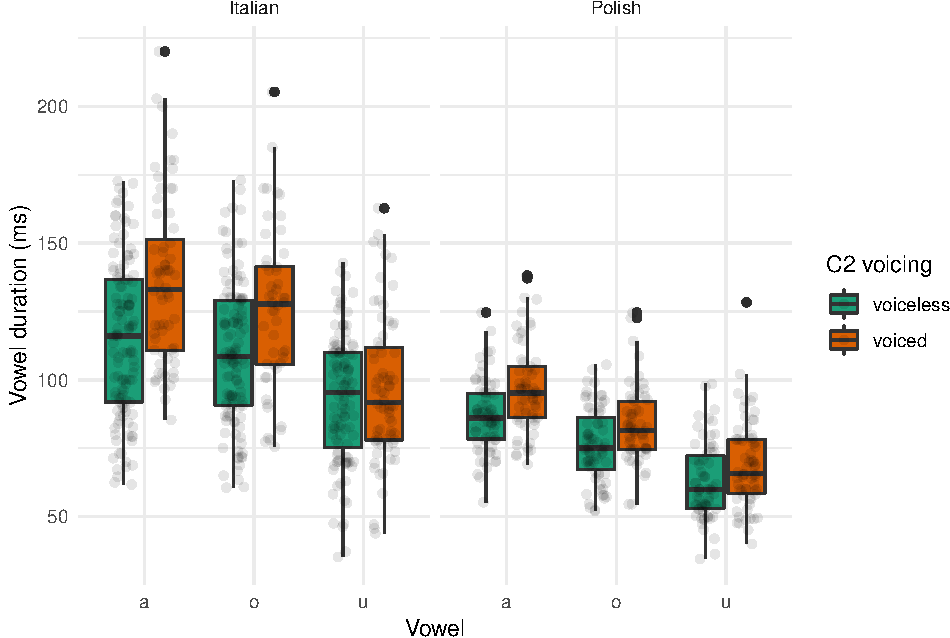
\includegraphics[width=\linewidth]{2018-jasa_files/figure-latex/vowels-plot-1} \caption{Raw data and boxplots of the duration in milliseconds of vowels in Italian (left) and Polish (right), for the vowels /a, o, u/ when followed by a voiceless (green) or voiced (orange) stop. }\label{f:vowels-plot}
\end{figure}

\Cref{f:vowels-plot} shows boxplots and raw data of vowel duration for
the three vowels /a, o, u/ when followed by voiceless or voiced stops in
Italian and Polish. Vowel tend to be longer when followed by a voiced
stop in both languages. The effect appears to be greater in Italian than
in Polish, especially for the vowels /a/ and /o/. There is no evident
effect of C2 voicing in /u/ in Italian, but the effect is discernible in
Polish /u/. In Italian, vowels have a mean duration of 106 ms (sd = 27)
before voiceless stops, and a mean duration of 118 ms (sd = 33) before
voiced stops. Polish vowels are on average 75 ms long (sd = 16) when
followed by a voiceless stop, and 83 ms long (sd = 19) if a voiced stop
follows. The difference in vowel duration based on the raw means is 12
ms in Italian and 8 ms in Polish.

A linear mixed-effects model with vowel duration as the outcome variable
was fitted with the following predictors: fixed effects for C2 voicing
(voiceless, voiced), C2 place of articulation (coronal, velar), vowel
(a, o, u), language (Italian, Polish), and speech rate (as syllables per
second); by-speaker and by-word random intercepts with by-speaker random
slopes for C2 voicing. All possible interactions between C2 voicing,
vowel, and language were included. The following terms are significant
according to \emph{t}-tests with Satterthwaite's approximation to
degrees of freedom: C2 voicing, vowel, language, and speech rate. Only
the interaction between C2 voicing and vowel is significant. Vowels are
19 ms longer (se = 4.4) when followed by a voiced stop (C2 voicing). The
effect of C2 voicing is smaller with /u/ (around 5 ms, \(\hat{\beta}\) =
-14.4 ms, se = 6). Polish has on average shorter vowels than Italian
(\(\hat{\beta}\) = -28 ms, se = 8), and the effect of voicing is
estimated to be about 11 ms (although note that the interaction between
language and C2 voicing is not significant). Speech rate has a negative
effect on vowel duration, such that faster rates correlate with shorter
vowel durations (\(\hat{\beta}\) = -15 ms, se = 1).

\subsection{Consonant closure
duration}\label{consonant-closure-duration}

\begin{figure}
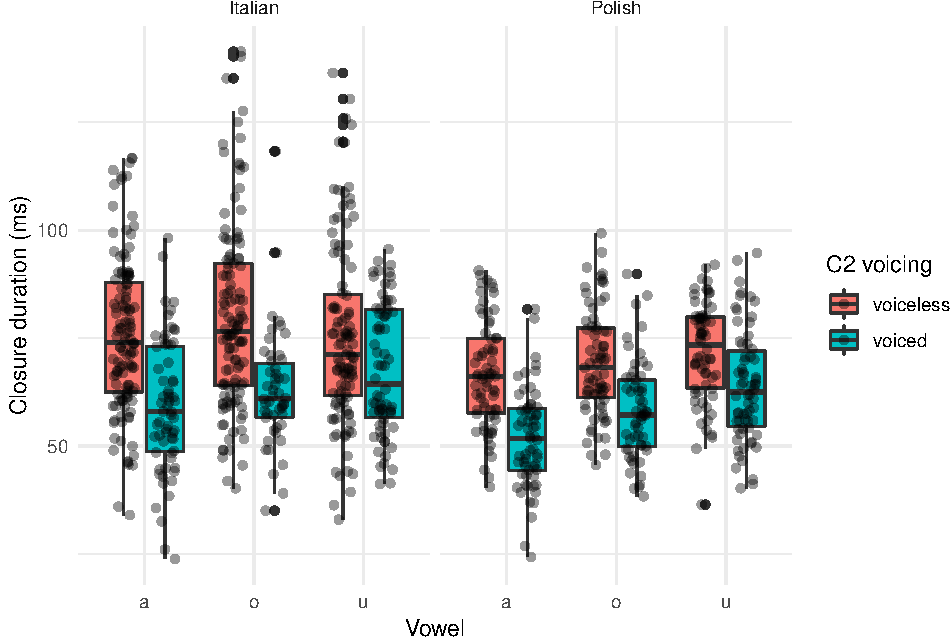
\includegraphics[width=\linewidth]{2018-jasa_files/figure-latex/closure-plot-1} \caption{Raw data and boxplots of closure duration in milliseconds of voiceless (green) and voiced (orange) stops in Italian (left) and Polish (right) when preceded by the vowels /a, o, u/.}\label{f:closure-plot}
\end{figure}

\Cref{f:closure-plot} illustrates stop closure durations with boxplots
and individual raw data points. A pattern opposite to that with vowel
duration can be noticed: closure duration is shorter for voiced than for
voiceless stops. The closure of voiceless stops in Italian is 77 ms long
(sd = 20), while the voiced stops have a mean closure duration of 63 ms
(sd = 15). In Polish, the closure duration is 69 ms (sd = 12) in
voiceless stops and 58 ms (sd = 13) in voiced stops. The difference in
closure duration based on the raw means is 14 ms in Italian and 11 ms in
Polish. The same model specification as with vowel duration has been
fitted with consonant closure duration as the outcome variable. C2
voicing, C2 place, and speech rate are significant. Stop closure is 16.5
ms shorter (se = 3) if the stop is voiced and 3.5 ms longer (se = 1.5)
if velar. Finally, faster speech rates correlate with shorter closure
durations (\(\hat{\beta}\) = -8.5 ms, se = 1 ms).

\subsection{Vowel and closure
duration}\label{vowel-and-closure-duration}

\begin{figure}
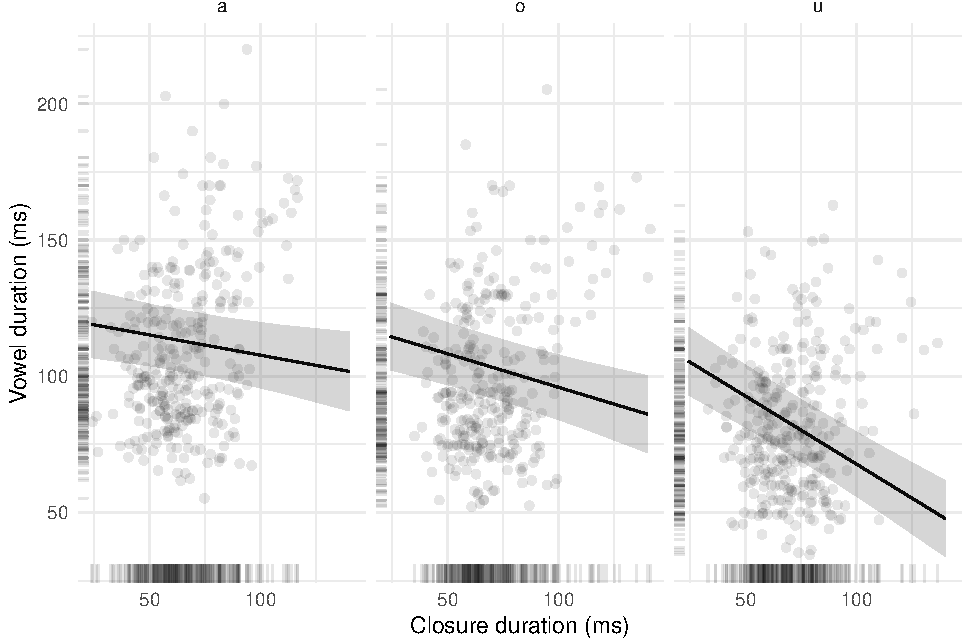
\includegraphics[width=\linewidth]{2018-jasa_files/figure-latex/vow-clo-plot-1} \caption{Raw data and estimated regression lines of the effect of closure duration on vowel duration for the vowels /a, o, u/ (from a mixed-effects model fitted to data pooled from Italian and Polish).}\label{f:vow-clo-plot}
\end{figure}

A model addressing the relationship between vowel and stop closure
duration was fitted with the following terms and interactions: vowel
duration as the outcome variable; as fixed effects, closure duration,
vowel, speech rate; an interaction between closure duration and vowel;
by-speaker and by-word random intercepts, and by-speaker random slopes
for C2 voicing. Closure duration has a significant effect on vowel
duration (\(\hat{\beta}\) = -0.15 ms, se = 0.06 ms). The effect with /u/
is greater than with /a/ and /o/ (\(\hat{\beta}\) = -0.35 ms, se = 0.06
ms). In general, closure duration is inversely proportional to vowel
duration. However, such correlation is quite weak, as shown by the small
estimates. A 1 ms increase in closure duration corresponds to a 0.2--0.5
ms decrease in vowel duration. \Cref{f:vow-clo-plot} shows for each
vowel /a, o, u/ the individual data points and the regression lines with
confidence intervals extracted from the mixed-effects model.

\subsection{Word duration}\label{word-duration}

Words with a voiceless C2 are on average 397 ms long (sd = 81) in
Italian and 356 ms long (sd = 39) in Polish. Words with a voiced stop
have a mean duration of 396 ms (sd = 72) in Italian and 362 ms (sd = 39)
in Polish. The following full and null models were fitted to test the
effect of C2 voicing on word duration. The full model is made up of the
following fixed effects: C2 voicing, C2 place, vowel, language, and
speech rate. The model also includes by-speaker and by-word random
intercepts, and a by-speaker random slope for C2 voicing. The null model
is the same as the full model with the exclusion of the fixed effect of
C2 voicing. The Bayes factor of the null against the full model is 24.
Thus, the null model (in which there is no effect of C2 voicing,
\(\beta\) = 0) is 24 times more likely under the observed data than the
full model. This indicates that there is strong evidence for a null
effect of C2 voicing on word duration.

\subsection{Release to Release interval
duration}\label{release-to-release-interval-duration}

\begin{figure}
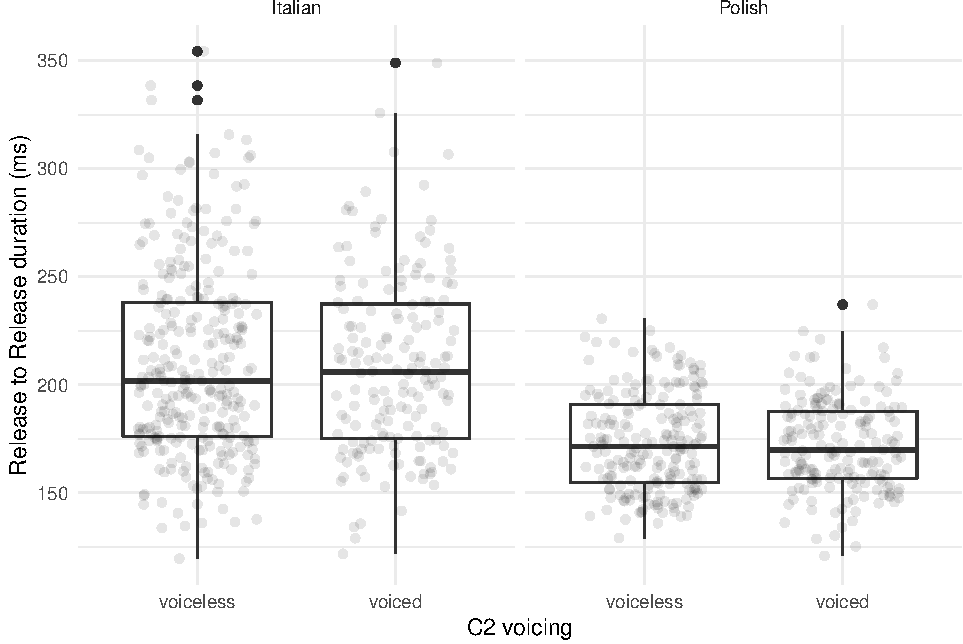
\includegraphics[width=\linewidth]{2018-jasa_files/figure-latex/rr-plot-1} \caption{Raw data and boxplots of the duration in milliseconds of the Release to Release interval in Italian (left) and Polish (right) when C2 is voiceless or voiced.}\label{f:rr-plot}
\end{figure}

In \Cref{f:rr-plot}, boxplots and raw data points show the duration of
the Release to Release interval in words with a voiceless vs.~a voiced
C2 stop, in Italian and Polish. It can be seen that the distributions,
medians, and quartiles of the durations in the voiceless and voiced
condition do not differ much in either language. In Italian, the mean
duration of the Release to Release interval is 210 ms (sd = 44) if C2 is
voiceless, and 209 ms (sd = 41) if voiced. In Polish, the mean durations
are respectively 173 (sd = 22) and 172 (sd = 21) ms. The specifications
of the null and full models for the Release to Release duration are the
same as for word duration. The Bayes factor of the null model against
the full model is 23, which means that the null model (without C2
voicing) is 23 times more likely than the model with C2 voicing as a
predictor. The data suggests there is positive evidence that duration of
the Release to Release interval is not affected by C2 voicing.

\subsection{Summary}\label{summary}

Seventeen participants were recorded while reading CV́CV words embedded
in a frame sentence. The stressed vowel was either /a, o, u/, and C2 was
one of /t, d, k, g/. Of the seventeen participants, 11 are native
speakers of Italian and 6 of Polish. Vowel, stop closure, word, and
Release to Release interval duration were measured from the acoustic
signal. The analyses of the durational data suggest that:

\begin{enumerate}[(a)]
  \item Stressed vowels in C\textsubscript{1}V́C\textsubscript{2}V words in Italian and Polish are 19 ms longer (se = 4.4) when C2 is voiced.
  \item C2 closure is 16.5 ms shorter (se = 3) if the stop is voiced.
  \item Vowel duration negatively correlates with closure duration, such that shorter closures correspond to longer vowels.
  \item Both word duration and Release to Release duration are not affected by the underlying voicing specification of C2.
\end{enumerate}

\section{Discussion}\label{discussion}

The data and statistical analyses of this exploratory study suggest that
the duration of the interval between the releases of two consecutive
consonants in CV́CV words (the Release to Release interval) is
insensitive to the phonological voicing of the second consonant (C2) in
Italian and Polish. In accordance with a compensatory temporal
adjustment account \citep{slis1969, lehiste1970}, the difference in
vowel duration before voiceless vs.~voiced stops can be seen as the
outcome of differences in stop closure duration. More specifically, the
timing of the closure onset of C2 within the invariant Release to
Release interval determines the duration of the preceding vowel. An
earlier closure onset relative to the onset of the preceding vowel (like
in the case of voiceless stops) causes the vowel to be shorter. On the
other hand, a later closure onset (like with voiced stops) produces a
longer vowel. \Cref{f:compensatory} illustrates this mechanism.

\begin{figure}
  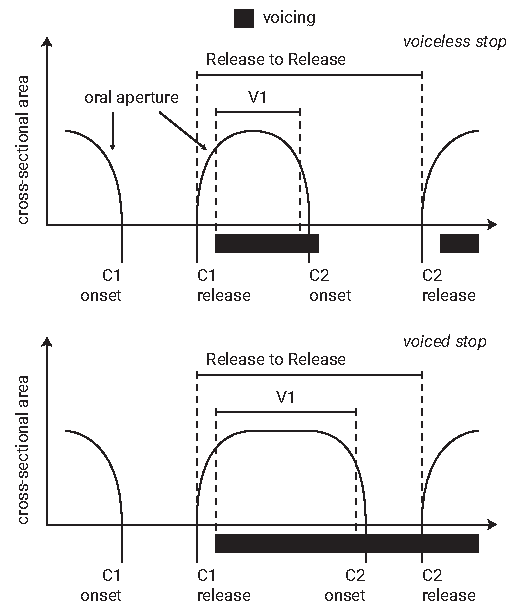
\includegraphics{img/compensatory.pdf}
  \caption{A schematic representation of the voicing effect as a compensatory temporal adjustment phenomenon. The schematic shows the gestural unfolding of a CV́C sequence when C2 is voiceless (top panel), or voiced (bottom panel). Oral cavity aperture (on the \textit{y}-axis, as the inverse of oral constriction) through time (on the \textit{x}-axis) is represented by the black line. Lower values represent a more constricted oral tract (a contoid configuration), while higher values indicate a more open oral tract (a vocoid configuration). The black bars below the time axis represent voicing (vocal fold vibration). Various landmarks and intervals are indicated in the schematic. Design based on \citet{esposito2002}.}
  \label{f:compensatory}
\end{figure}

The invariance of the Release to Release interval allows us to refine
the logistics of the compensatory account by narrowing the scope of the
temporal adjustment action. A limitation of this account, as proposed by
\citet{slis1969} and \citet{lehiste1970}, is the lack of a precise
identification of the word-internal mechanics of compensation. As
already discussed in \Cref{s:intro}, it is not clear, for example, why
the adjustment should target the preceding stressed vowel, rather then
the following unstressed vowel or any other segment in the word. Since
the Release to Release interval includes just the vowel (broadly defined
as a vocoid gesture) and the consonant closure, it follows that
differences in closure duration must be reflected in differences in the
duration of the preceding vowel.

On the one hand, the voicing effect can be re-interpreted as a
by-product of gestural timing, rather then a consequence of intrinsic
features of voicing \emph{per se}, with a constant Release to Release
interval as the explanans. On the other hand, the Release to Release
invariance is in turn an explanandum. In the following section, I offer
a gestural organisation account that allows the invariance of such
interval to follow from the relative timing of the articulatory gestures
in a CV́C sequence.

\subsection{Gestural alignment}\label{gestural-alignment}

\label{s:gestural}

\begin{figure}
  \centering
  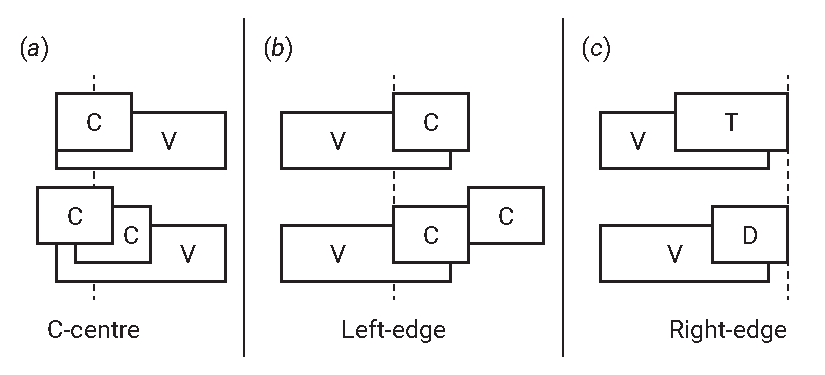
\includegraphics[width=\linewidth]{img/gorganisation.pdf}
  \caption{Gestural organisation patterns for onsets (a), codas (b), heterosyllabic onsets (c). C = consonant, V = vowel, T = voiceless stop, D = voiced stop. See \Cref{s:gestural} for details. Based on \citet{marin2010}.}
  \label{f:gorganisation}
\end{figure}

According to the coupled oscillator model of syllabic structure
\citep{browman1988, browman2000, goldstein2006, goldstein2014},
articulatory gestures can be timed according to two coupling modes:
in-phase (synchronous) mode, by which two gestures start in synchrony,
or anti-phase (sequential) mode, in which a gesture starts when the
preceding one has reached its target. \citet{marin2010} showed that
onset consonants in American English are in-phase with respect to the
vowel nucleus and anti-phase with each other. Such phasing pattern
establishes a stable relationship between the centre of the consonant
(or consonants in a cluster) and the following vowel. Independent of the
number of onset consonants, the temporal midpoint of the onset (the
so-called `C-centre') is maintained at a fixed distance from the vowel,
such that an increasing number of consonants in the onset does not
change the distance between the vowel and the onset C-centre
(\Cref{f:gorganisation}a). On the other hand, coda consonants are timed
anti-phase with the preceding vowel and between themselves. Temporal
stability in codas is found in the lag between the vowel and the
left-most edge of the coda, which is not affected by the number of coda
consonants (\Cref{f:gorganisation}b). Other studies found further
evidence for the synchronous and sequential coupling modes (see
extensive review in \citealt{marin2010} and \citealt{marin2014}),
although the use of one mode over the other depends on the language and
the consonants under study.

Consonants can thus be said to follow either a C-centre or a left-edge
organisation pattern. In both cases, of course, the pattern is relative
to the tautosyllabic vowel (the following vowel for onsets, the
preceding vowel for codas). To the best of my knowledge, no study has
reported the timing of onset consonants relative to the \emph{preceding}
(heterosyllabic) vowel. The results from this acoustic study on Italian
and Polish are compatible with a right-edge organisation pattern for
onset consonants relative to the preceding stressed vowel
(\Cref{f:gorganisation}c). In CV́CV words, the timing of the C2 release
(the acoustic parallel of the articulatory right edge of C2) is fixed
relative to V1.

A consequence of a right-edge organisation pattern of C2 relative to V1
in CV́CV words is that differences in C2 closure duration do not affect
the lag between V1 and the release of C2, as shown by the results of
this study. The invariance of the lag between the release of C1 and that
of C2 then can be seen to follow from the invariance in timing between,
on the one hand, C1 (which is always /p/ in this study) and V1, and, on
the other, between V1 and the right edge of C2.

A right-edge organisation account is compatible with findings from a
variety of sources. \citet{celata2018} show with ultrasound tongue
imaging data that, in Italian, vowels followed by single consonants are
longer than when followed by geminates (for example, /ba.ta/ vs.
/bat.ta/). However, vowels followed by a tautosyllabic cluster have the
same duration as vowels followed by a heterosyllabic cluster (/pa.tron/
vs. /bat.man/). \citet{celata2018} argue that these results corroborate
a rhythmic account in which the relevant unit is not the traditional
syllable, but rather the the VC(C) sequence. The importance of the VC(C)
sequence as relevant speech unit has been previously recognised in the
work of \citet{farnetani1986} (who called it the `rhythmic syllable')
and \citet{steriade2012} (who uses the term `vowel to vowel interval',
see also \citealt{hirsch2014} and \citealt{lunden2017}). The duration of
the rhythmic syllable or interval is constant across the phonological
contexts, while the duration of the traditional syllable is not. This
reflects a gestural organisation in which the timing of the right edge
of the consonant is fixed relative to the vowel.

\citet{de-jong1991} reports that the closing gesture of voiceless stops
(following stressed vowels) is faster than that of voiced stops, and
that also it is timed earlier with respect to the opening gesture of the
stressed vowel. According to \citet{de-jong1991}, the differences in
vowel duration are driven by the timing of the consonantal closing
gesture relative to the vocalic opening gesture (also see
\citealt{hertrich1997}). Moreover, the data in \citet{de-jong1991} show
that the final portion of the opening gesture is prolonged before voiced
stops.

This pattern fits the one reported in an electromyographic study by
\citet{raphael1975}. The electromyographic signal corresponding to the
vocalic gesture reaches its plateau at the same time relative to the
preceding consonant in the voiceless and voiced context, but the plateau
is held for longer in the case of vowels followed by voiced stops. This
indicates that muscular activation in the vocalic gesture before voiced
stops is held for longer. \citet{raphael1975} further notes that the
durational difference in muscular activation corresponds to the
difference in the acoustic duration of vowels before voiceless
vs.~voiced stops (see also \citealt{warren2005}).

The results of the studies just discussed, together with the results
from this study, bring support to a view in which two aspects of
gestural organisation contribute to the difference in vowel duration
observed before consonants varying in their voicing specification. These
aspects are: (1) the \emph{right-edge alignment} of coda consonants
following a stressed vowel relative to the latter, and (2) the
\emph{differential timing of the closing gesture onset} for voiceless
vs.~voiced stops. The interplay of these two aspects can be synthesised
into a compensatory temporal adjustment account, which requires a
temporally constant interval, produced by (1), and a temporal
reorganisation, brought about by (2).

\subsection{Limitations and future
work}\label{limitations-and-future-work}

The generalisations put forward in this paper strictly apply to
disyllabic words with a stressed vowel in the first syllable. It is
possible that the organisation pattern found in this context does not
occur in sequences including an unstressed vowel. For example, it is
known that the difference in closure duration between voiceless and
voiced stops is not stable when the stops precede a stressed vowel,
although vowels preceding pre-stress stops have slightly different
durations \citep{davis1989}. According to the gestural interpretation
given here, the absence of differences in closure duration should
correspond to no difference in vowel duration. Data from different
contexts and different languages is thus needed to assess the generality
of the claims put forward in this paper.

The constraints on experimental material enforced by the use of
ultrasound tongue imaging have been previously mentioned in
\Cref{s:materials}. Given these constraints, temporal information from
other vowels (like front vowels) and places of articulation is a
desideratum. \Cref{s:gestural} discusses the interpretation of the
Release to Release invariance in CV́CV words as a consequence of the
timing of C2 rather than of a holistic CV́C motor plan in which the
Release to Release interval is held constant. Although beyond the scope
of this paper, disambiguating between these two interpretations on
articulatory grounds is fundamental for a general understanding of a
theory of gestural organisation (a promising venue of research might be
the activation-spin model by \citealt{tilsen2013}).

The compensatory temporal adjustment account presented here extends to
other durational effects discussed in the literature. In particular, the
account bears predictions on the direction of the durational difference
led by phonation types different from voicing, like aspiration and
ejection. For example, the mix of results with regard to the effect of
aspiration \citep{durvasula2012} suggests that the conditions for a
temporal adjustment might differ across the contexts and languages
studied. In light of the results in \citet{begus2017}, future studies
will have to investigate the durational invariance of speech intervals
in relation to a variety of phonation contrasts.

\section{Conclusion}\label{conclusion}

The results of an exploratory study on the effect of voicing on vowel
duration bring support for a compensatory temporal adjustment account of
such effect. Acoustic data from seventeen speakers of Italian and Polish
show that the temporal distance between two consecutive stop releases is
not affected by the voicing of the second stop in CV́CV words. The
temporal invariance of the Release to Release interval, together with a
difference in stop closure duration of voiceless and voiced stops,
causes vowels to be shorter when followed by voiceless stops (which have
a long closure) and longer when followed by voiced stops (the closure of
which is short). I proposed that the Release to Release invariance is a
consequence of the gestural organisation of the CV́C sequence, in which
the lag between the right-edge of the second consonant and the preceding
stressed vowel is fixed.

\appendix

\section{Output of statistical
models}\label{output-of-statistical-models}

\label{a:stats}

See \Cref{tab:vow-table}, \Cref{tab:clo-table}, and
\Cref{tab:vow-clo-table}.

\begin{table}

\caption{\label{tab:vow-table}Summary of the linear mixed-effects model fitted to vowel duration.}
\centering
\begin{tabular}[t]{lrrrrrrrl}
\toprule
term & Estimate & SE & CI low & CI up & df & t-value & p-value & < α\\
\midrule
Intercept & 202.5289 & 8.6169 & 185.6400 & 219.4178 & 134.7948 & 23.5036 & 0.0000 & *\\
C2 voi: voiced & 18.9669 & 4.3898 & 10.3631 & 27.5707 & 12.7785 & 4.3207 & 0.0009 & *\\
Vow: /o/ & -6.1457 & 3.9512 & -13.8899 & 1.5985 & 8.6900 & -1.5554 & 0.1555 & \\
Vow: /u/ & -26.3039 & 3.9772 & -34.0991 & -18.5087 & 8.9199 & -6.6136 & 0.0001 & *\\
Lang: Polish & -24.2194 & 8.1708 & -40.2338 & -8.2050 & 21.7230 & -2.9642 & 0.0072 & *\\
\addlinespace
C2 place: velar & -8.1827 & 1.6984 & -11.5116 & -4.8539 & 10.5938 & -4.8178 & 0.0006 & *\\
Syl. rate & -15.2920 & 1.2679 & -17.7771 & -12.8070 & 775.7483 & -12.0608 & 0.0000 & *\\
Voiced, /o/ & -2.0453 & 5.8662 & -13.5428 & 9.4522 & 10.5314 & -0.3487 & 0.7342 & \\
Voiced, /u/ & -14.4536 & 5.8040 & -25.8292 & -3.0780 & 10.0977 & -2.4903 & 0.0318 & *\\
Voiced, Polish & -7.9928 & 6.4252 & -20.5860 & 4.6005 & 14.2528 & -1.2440 & 0.2336 & \\
\addlinespace
/o/, Polish & -3.6121 & 5.7389 & -14.8601 & 7.6360 & 9.6704 & -0.6294 & 0.5437 & \\
/u/, Polish & 1.6149 & 5.7695 & -9.6931 & 12.9230 & 9.8777 & 0.2799 & 0.7853 & \\
Voiced, /o/, Polish & -2.9987 & 8.3627 & -19.3894 & 13.3920 & 10.8862 & -0.3586 & 0.7268 & \\
Voiced, /u/, Polish & 7.9601 & 8.3077 & -8.3227 & 24.2428 & 10.6040 & 0.9582 & 0.3593 & \\
\bottomrule
\end{tabular}
\end{table}

\begin{table}

\caption{\label{tab:clo-table}Summary of a linear mixed-effects model fitted to closure duration.}
\centering
\begin{tabular}[t]{lrrrrrrrl}
\toprule
term & Estimate & SE & CI low & CI up & df & t-value & p-value & < α\\
\midrule
Intercept & 119.7338 & 7.2100 & 105.6023 & 133.8652 & 128.2742 & 16.6065 & 0.0000 & *\\
C2 voi: voiced & -16.5825 & 4.3129 & -25.0356 & -8.1294 & 17.8144 & -3.8449 & 0.0012 & *\\
Vow: /o/ & 3.6830 & 3.4951 & -3.1672 & 10.5333 & 9.0918 & 1.0538 & 0.3192 & \\
Vow: /u/ & -1.9898 & 3.5174 & -8.8837 & 4.9041 & 9.3243 & -0.5657 & 0.5849 & \\
Lang: Polish & -6.9400 & 6.8688 & -20.4027 & 6.5226 & 22.0443 & -1.0104 & 0.3233 & \\
\addlinespace
C2 place: velar & 3.4024 & 1.4976 & 0.4672 & 6.3376 & 10.9532 & 2.2719 & 0.0443 & *\\
Syl. rate & -8.4278 & 1.0550 & -10.4954 & -6.3601 & 557.6472 & -7.9887 & 0.0000 & *\\
Voiced, /o/ & 1.1040 & 5.1738 & -9.0364 & 11.2445 & 10.8916 & 0.2134 & 0.8350 & \\
Voiced, /u/ & 9.9882 & 5.1257 & -0.0581 & 20.0344 & 10.4981 & 1.9486 & 0.0786 & \\
Voiced, Polish & 1.6759 & 6.5019 & -11.0675 & 14.4194 & 20.0145 & 0.2578 & 0.7992 & \\
\addlinespace
/o/, Polish & -0.2681 & 5.0672 & -10.1997 & 9.6635 & 10.0440 & -0.0529 & 0.9588 & \\
/u/, Polish & 7.1432 & 5.0932 & -2.8393 & 17.1256 & 10.2505 & 1.4025 & 0.1903 & \\
Voiced, /o/, Polish & 1.5022 & 7.3707 & -12.9441 & 15.9485 & 11.2269 & 0.2038 & 0.8422 & \\
Voiced, /u/, Polish & -3.2088 & 7.3279 & -17.5711 & 11.1536 & 10.9696 & -0.4379 & 0.6700 & \\
\bottomrule
\end{tabular}
\end{table}

\begin{table}

\caption{\label{tab:vow-clo-table}Summary of a linear mixed-effects model fitted to vowel duration with closure duration as predictor.}
\centering
\begin{tabular}[t]{lrrrrrrrl}
\toprule
term & Estimate & SE & CI low & CI up & df & t-value & p-value & < α\\
\midrule
Intercept & 219.3142 & 10.4477 & 198.8371 & 239.7913 & 123.5512 & 20.9917 & 0.0000 & *\\
C2 closure & -0.1487 & 0.0632 & -0.2726 & -0.0249 & 50.3807 & -2.3532 & 0.0226 & *\\
Vow: /o/ & -2.0462 & 5.4702 & -12.7675 & 8.6751 & 81.5530 & -0.3741 & 0.7093 & \\
Vow: /u/ & -5.0236 & 5.5582 & -15.9176 & 5.8703 & 86.7938 & -0.9038 & 0.3686 & \\
Syl. rate & -17.5364 & 1.2855 & -20.0559 & -15.0168 & 896.1529 & -13.6415 & 0.0000 & *\\
\addlinespace
C2 closure, /o/ & -0.0973 & 0.0615 & -0.2178 & 0.0231 & 876.5971 & -1.5835 & 0.1137 & \\
C2 closure, /u/ & -0.3500 & 0.0619 & -0.4712 & -0.2288 & 895.3921 & -5.6582 & 0.0000 & *\\
\bottomrule
\end{tabular}
\end{table}

\section{Socio-linguistic information of
participants}\label{socio-linguistic-information-of-participants}

\label{a:socioling}

See \Cref{t:socio}.

\ctable[caption = Participants' sociolinguistic information.,
label = t:socio,
width=\textwidth,
star,
doinside = \footnotesize
]{llll>{\raggedright}p{5cm}lll}{}{
\FL
ID & Age & Sex    & Native L & Other Ls& City of birth & Spent most time in & > 6 mo \ML
it01 & 29 & Male   & Italian & English, Spanish                          & Verbania            & Verbania        & Yes \NN
it02 & 26 & Male   & Italian & Friulian, English, Ladin-Venetan          & Udine               & Tricesimo & Yes \NN
it03 & 28 & Female & Italian & English, German                           & Verbania            & Verbania        & No  \NN
it04 & 54 & Female & Italian & Calabrese                                 & Verbania            & Verbania        & No  \NN
it05 & 28 & Female & Italian & English                                   & Verbania            & Verbania        & No  \NN
it09 & 35 & Female & Italian & English                                   & Vignola & Vignola         & Yes \NN
it11 & 24 & Male   & Italian & English                                   & Monza               & Monza           & Yes \NN
it13 & 20 & Female & Italian & English, French, Arabic, Farsi            & Ancona              & Chiaravalle     & Yes \NN
it14 & 32 & Male & Italian & English, Spanish & Frosinone & Frosinone & Yes \NN
pl02 & 32 & Female & Polish  & English, Norwegian, French, German, Dutch & Koło                & Poznań          & Yes \NN
pl03 & 26 & Male   & Polish  & Russian, English, French, German          & Nowa Sol            & Poznań          & Yes \NN
pl04 & 34 & Female & Polish  & Spanish, English, French                  & Warsaw              & Warsaw          & No  \NN
pl05 & 42 & Male   & Polish  & English, French                           & Przasnysz           & Warsaw        & No  \NN
pl06 & 33 & Male   & Polish  & English                                   & Zgierz              & Zgierz          & Yes \NN
pl07 & 32 & Female & Polish  & English, Russian                          & Bielsk Podlaski     & Bielsk Podlaski & Yes \LL
}

\section{Target words}\label{target-words}

\label{a:targets}

See \Cref{t:targets}.

\ctable[caption = Target words.,
label = t:targets,
star,
doinside = \footnotesize
]{lllllll}{}{
\FL
Italian   &        &      & \hspace{0.5cm} & Polish &      &      \NN
\cmidrule{1-3}\cmidrule{5-7}
pata      & poto*  & putu & & pata   & poto & putu \NN
pada      & podo   & pudu & & pada*  & podo & pudu \NN
paca*     & poco*  & pucu & & paka*  & poko & puku \NN
paga*     & pogo   & pugu & & paga   & pogo & pugu \LL
}

%% before appendix (optional) and bibliography:
% \begin{acknowledgments}
%This research was supported by  ...
% \end{acknowledgments}

% -------------------------------------------------------------------------------------------------------------------
%   Appendix  (optional)

%\appendix
%\section{Appendix title}

%If only one appendix, please use
%\appendix*
%\section{Appendix title}


%=======================================================
%IMPORTANT

%Use \bibliography{<name of your .bib file>}+
%to make your bibliography with BibTeX.

%Once you have used BibTeX you
%should open the resulting .bbl file and cut and paste the entire contents
%into the end of your article.
%=======================================================

\bibliography{linguistics.bib}


\end{document}
